\documentclass[10pt]{article}
\usepackage[breaklinks=true]{hyperref}
\usepackage[margin=0.75in]{geometry}

\usepackage{textcomp}

\usepackage{color}
\usepackage{graphicx}
\definecolor{pblue}{rgb}{0.13,0.13,1}
\definecolor{pgreen}{rgb}{0,0.5,0}
\definecolor{pred}{rgb}{0.9,0,0}
\definecolor{pgrey}{rgb}{0.46,0.45,0.48}

\usepackage{listings}
\lstset{language=bash,
  showspaces=false,
  showtabs=false,
  breaklines=true,
  showstringspaces=false,
  tabsize=2,
  breakatwhitespace=true,
  commentstyle=\color{pgreen},
  keywordstyle=\color{pblue},
  stringstyle=\color{pred},
  numbers=left,
  stepnumber=1,
  basicstyle=\small\ttfamily,
  frame=single,
  moredelim=[il][\textcolor{pgrey}]{$$},
  moredelim=[is][\textcolor{pgrey}]{\%\%}{\%\%}
}

\title{\textbf{Week 09} \\
\LARGE Apache2 and Flask \\
\Large Making a Professional Webserver}
\author{
	Melvyn Ian Drag
}
\date{\today}


\begin{document}
\maketitle

\begin{abstract}
Last class we took a look at the toy `SimpleHTTPServer' in Python3. Tonight we'll use a real website backend - Flask - and we'll server content on a real server - Apache2. As before, we'll make \textbf{GET} and \textbf{POST} requests using the command line tool cURL.
\end{abstract}

\section{Meta Data}
I want to show you how to set up a webserver on Linux - last week's lecture was supposed to ease you into the mindset, but a few people missed lecture or left early. There isn't time to revist last week's lecture, there was too much information. Hopefully today will stand alone. If it doesn't, you'll need to work through last week's notes. There was a 3 hour lecture, so you will probably need at least 3 hours to read through the notes.

Still, we'll try and make tonight as `stand-alone' as possible.

\section{What's a Webserver?}
The term is overloaded. A server is a computer, connected to a network, that other computers can access. There may be more ways to define it, but that's what I think of. But for your midterm I had you install some postgresql server stuff. In that case I was referring to the database server software. And tonight I'm going to refer to Apache2 as a 'webserver' - it's actually software that runs \textit{on} a webserver, which is the machine. It's just that the terms are overloaded.

\section{What's Flask?}
Flask is what is called a \textbf{Library}. It's some code that you can use in a language to solve a particular problem. For example, if you know Java you've probably used the \textit{java.util} library for things like \textit{ArrayList}s. In Python last week we used a library calle \textit{SimpleHTTPServer} to serve up some webpages for us on the address \textit{localhost:8000}.

\section{What's a REST API}
There are just too many buzzwords out there. I've showed you that we could get html back with curl when we curled out own little python server. Then I showed you that when we curled api.github.com, we got back JSON data. There is more to it, but in general, when we send and receive JSON, we call this a REST API. If you look into web development more, you'll  learn what the REST stand for, and then you'll learn why RESTful ness is important. For us it doesn't matter at all. All that matters is that you can see that REST is for exchanging JSON data.

\subsection{Job interview prep}
\noindent\textit{\textbf{Interviewer:} I see you know a bit about Linux webserver maintenance. Do you know what a REST API is?}

\noindent \textbf{You: } Honestly, not too much because I'm not a webdeveloper. But I do know that REST APIs are very popular now, and they typically involve the exchange of JSON data. JSON data is when the data is structured like a Python dicitonary, or a Java Hashmap  - its a bunch of key-value pairs in curly braces.

If you can give the above answer, you'll know enough for now.

\section{Back to Tabs and Spaces}
We briefly mentioned the difference between tabs and spaces. You can set the tab width in Vim. Maybe mention the ASCII codes for tab vs space so that the folks in the Java class can make the connection.


\section{What we'll do today}
Today we'll bring a real website online. Last week we made a trivial website with Python's SimpleHTTPServer, but today we're going to use a real, professional-grade server ( Apache2 ) and a real backend web framework ( Flask ). There are other servers like NGINX and there are other backend webframeworks like Django, Play, Spring, Ruby on Rails, etc., I've just chosen this pair because it's the easiest to code of the few things I know. Spring on NGINX would be considerably harder to configure.

\begin{figure}[h]
  \centering
    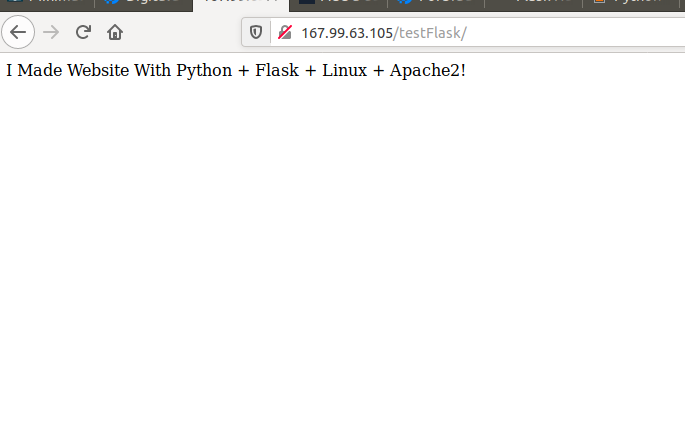
\includegraphics[width=0.8\textwidth]{Exercise1Success.png}
  \caption{A website running on my server at IP address http://167.99.63.105/testFlask/}
\end{figure}



\section{Setting up server}
Get a debian 10 server

\begin{lstlisting}
root@machine$ apt update
root@machine$ apt install apache2
root@machine$ apt-get install libapache2-mod-wsgi-py3 python3-dev python3-pip
root@machine$ pip3 install flask flask-restful
root@machine$ apt install curl
root@machine$ service apache2 status
# should report that apache2 is running
root@machine$ curl localhost
# lots of data
root@machine$ curl localhost > curlResponse.html
# dump the data to a file so it's easier to look through
root@machine$ less curlResponse.html # look through, verify you have the default apache page. That means the server is running.
root@machine$ curl ipinfo.io/io # get your server ip address
\end{lstlisting}

Open a browser on a laptop or computer. Go to the server ip address, make sure the server is running. You should see the same default apache page you saw with curl localhost. But now you are looking at it through a browser on a different machine ( you ran curl on the webserver itself ).

\begin{figure}[h]
  \centering
    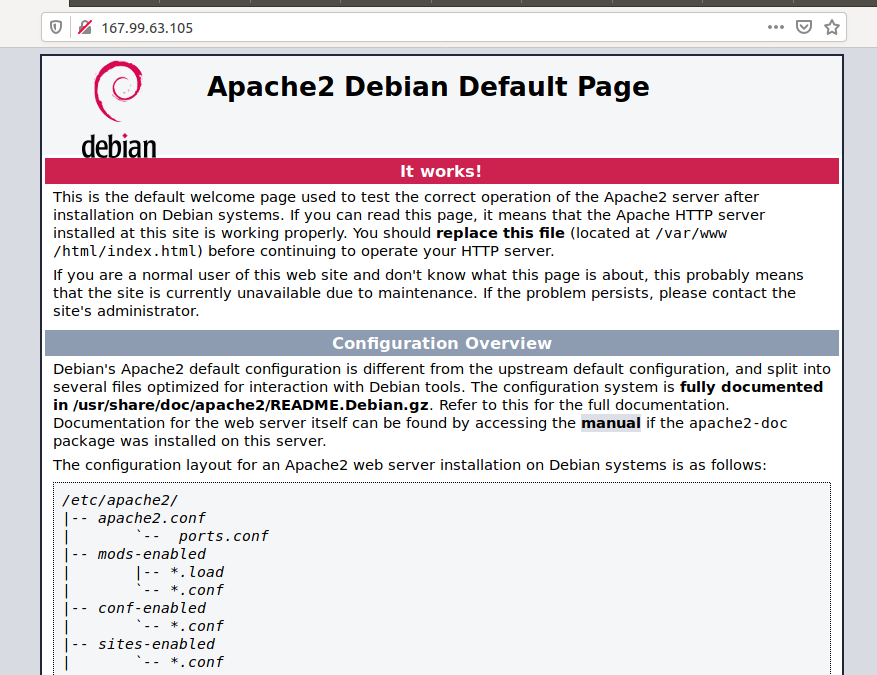
\includegraphics[width=0.8\textwidth]{defaultApache.png}
  \caption{default webpage provided by a fresh Apache2 install}
\end{figure}

So we've installed all the software we need! That was easy. Now we can build a little website and then connect the website code to the apache server we just installed and activated.

\section{Creating a Flask application}
The first thing we need to do is create a non root user for managing this stuff. We'll give the user sudo permission for the few root things we need to do to bring the website online. I've created user `webdeveloper'. You should do the same so you can copy and paste the code I've provided. If you create a different username, you'll need to make the minor modifications to make everyting match up.

\begin{lstlisting}
root@machine$ adduser webdeveloper
root@machine$ usermod -a -G sudo webdeveloper
root@machine$ sudo su - webdeveloper
root@machine$ mkdir /home/webdeveloper/ExampleFlask
\end{lstlisting}

Inside the ExampleFlask directory, put the files described below. Note that these files are available in the Example1/ExampleFlask directory in the class Git repo.

\subsection{\_\_init\_\_.py}
This is an empty file

\subsection{my\_flask\_app.py}
\lstinputlisting{Example1/ExampleFlask/my_flask_app.py}

\subsection{my\_flask\_app.wsgi}
\lstinputlisting{Example1/ExampleFlask/my_flask_app.wsgi}


\section{Connect Flask to Apache2}
Now we need to wire up our Flask application to the Apache webserver software. You will need to know your machine's ip address. I showed you a website you can curl that will tell you your ipaddress

\begin{lstlisting}
user@machine$ curl ipinfo.io/ip
# returns your external ip address
\end{lstlisting}

Then you need to create this file, and put the proper ip address. Note that you'll need to run vim with sudo as this is a privileged file.

\subsection{/etc/apache2/sites-available/ExampleFlask.conf}

\lstinputlisting{Example1/ExampleFlask.conf}

\subsection{Turn on and Test the Website}
Run these commands as the user `webdeveloper'
\begin{lstlisting}
webdeveloper@machine$ sudo a2ensite ExampleFlask
webdeveloper@machine$ sudo a2enmod wsgi
webdeveloper@machine$ sudo service apache2 restart
\end{lstlisting}

Then, open a browser on your laptop or the NJCU PC in front of you and go to 

\begin{center}
\textit{my.ip.addr.ess/testFlask}
\end{center}

You should see a message saying you've made your first website with Linux, flask, apache and python. You can share the link to show off your website to your friends and family! You could now also go to godaddy or namecheap, buy a domain name, and wire that up to your server so people can go to website.com instead of a scary looking ip address.


\section{Example2: Serving HTML}

\section{sed}


\section{Recap of what you know}
\begin{enumerate}
\item A bit about the Bash programming language
\item grep \& regular expressions
\item What a user is on Linux
\item What a group is on Linux
\item What is git?
\item You're comfortable using a command line interface now
\item There are a few different languages on the command line - we've used bash and dash
\item What permissions are and how to modify them
\item What is a root user
\item What is a process
\item What is a job
\item How to send signals to processes ( kill, CTRL+C, CTRL+Z )
\item How to make code ignore or block signals
\item How to install software on Linux
\item A cool trick for using setuid / setgid to make a non-root user do some root stuff
\item basics of relational dbs and how to configure one on Linux
\item What is cron
\item curl
\item some vocabulary like API, REST, regex, SQL, DB
\item A bit about python programming
\item What is a website backend? Set up a website backend with Apache2 + Flask
\item What is sed?
\end{enumerate}

\section{Coming Up In This Class}

We have a few more important things to cover
\begin{enumerate}
\item set up a git server
\item add a gitlab front end to the git server
\item Linux and Text encodings
\item xxd, everyone's favorite binary packet analyzer
\item The AWK programming language
\item The hows and whys of formatting harddrives, usb sticks, solid state drives, etc.
\item Encryption with gpg + pgp. How it relates to ssh and other pub/priv key schemes.
\end{enumerate}

\end{document}
